\section{Incremental Workflow Mining with Petri Nets}
Another relevant to my research approach to the process discovery developed by Rubin et al. \cite{citeulike:1885717} and van der Aalst et al \cite{citeulike:3718014} is called \textit{incremental workflow mining}. Authors not only designed sophisticated algorithms but built a software system using a business process mining framework ProM by van Dongen et al. \cite{citeulike:5043673} which synthesizes a Petri Net corresponding to the process observed. 
The system was tested on the SCM logs and while the process artifacts retrieved from SCM system are rather high-level, the approach discussed is very promising for the modeling of software processes from the low-level product and process data.

\begin{figure}[tbp]
   \centering
   \includegraphics[height=65mm]{petri.eps}
   \caption{Illustration of the ``Generation and Synthesis Approach'' from \cite{citeulike:5043673}: a) Transition System with regions shown; b),c) Petri Nets synthesized from the Transition System.}
   \label{fig:petri}
\end{figure}

Within the incremental workflow mining framework the input data from SCM audit trail information is mapped the event chain which corresponds to the software process artifacts. Authors call this process as \textit{abstraction on the log level} which is implemented as a set of filters which not only aggregate basic events into the single high-level entities but also remove irrelevant to the mining process information (noise). 

The event chain constructed through the abstraction then treated with the \textit{Generate} part of the \textit{``Generate and Synthesis''} \cite{citeulike:3718014} algorithm in order to generate a \textit{Transition System} which represents order of events. This algorithm looks at the history (prefix) and the future (suffix) sequences of events related to the current one in order to discover transitions.  When applied to the abstracted log information these algorithm is generating a rather large Transition System graph where edges are connecting abstracted events. This transition system then successively simplified by using various reduction strategies such as ``Kill Loops'', ``Extend'', ``Merge by Output'' and others; it is possible to combine these reduction strategies in order to achieve a greater simplification.

At the last step of the incremental workflow mining approach Transition Systems are used to \textit{Synthesize} labeled Petri nets (where different transition can refer to the same event) with the help of the \textit{``regions theory''} \cite{citeulike:5128170}. As with the Transition System generation authors tackling many different strategies of Petri nets synthesis showing great variability of the results achieved as shown at the Figure \ref{fig:petri}.

The great contribution of the incremental workflow mining is in the generality of methods used. It was shown that by tuning the ``Generate'' and ``Synthesize'' phases it is possible to tailor algorithm to the wide variety of processes. In particular, as mentioned before, Rubin et al. successfully applied this framework to the SCM logs analysis.